\chapter{Introduction}

This manual aims to get new users started with the Odin 2 synthesizer plugin and provide a detailed documentation for experienced users.

\section{Installation}
You can download the Odin 2 from \url{https://www.thewavewarden.com/odin2}. Make sure to download the correct installer for your platform.

\vspace{3mm}
\fat{Windows}:

The installation wizards will guide you through the process on Windows system.

\vspace{3mm}
\fat{MacOS}:

The installation wizard gives you the option to install either the VST3 or AudioUnit plugins. Installing the AudioUnit version is only recommended for users of Apples Digital Audio Workstation "Logic".

\vspace{3mm}
\fat{GNU/Linux}

For GNU/Linux based systems you have two options: Debian based operating systems (Debian, Ubuntu, Mint and many more) can use the convenient debian packages (.deb file) to install Odin. Other distributions have to use the manual installer. Open the README.txt file in the zip for further installation instructions in that case.

\vspace{5mm}
\begin{tcolorbox}[colback=yellow!10!white,
    colframe=white!20!black,
    center,
    valign=top,
    halign=left,
    center title,
    width=\textwidth]

    Please note that \fat{Odin 2 is not available as a 32Bit plugin} due to build complications.
    
    Furthermore,\fat{ Odin 2 is not available as a VST2 plugin} due to the ended licensing on behalf of Steinberg Media Technologies.
\end{tcolorbox}
\clearpage
\section{Overview}
\begin{center}
    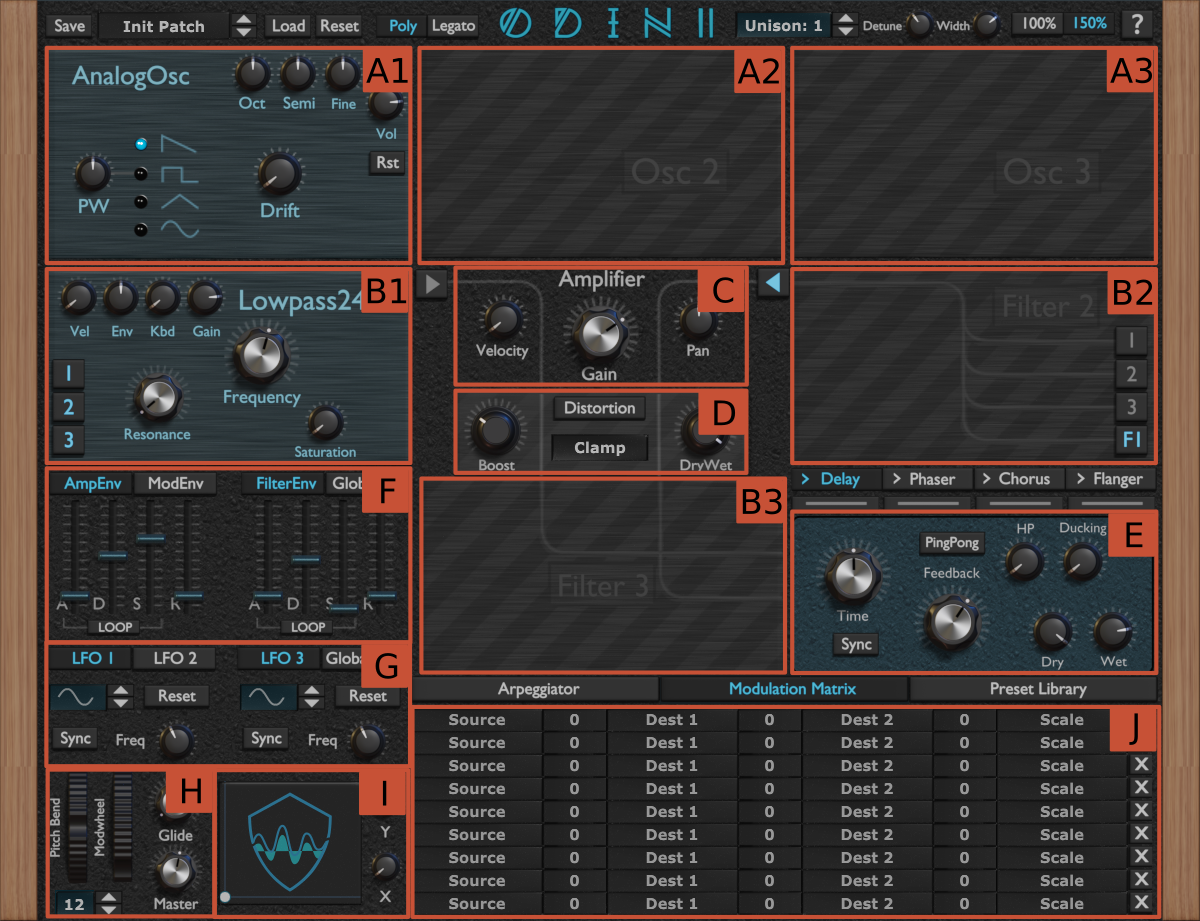
\includegraphics[width=\textwidth]{graphics/overview.png}
\end{center}

\begin{itemize}
    \item \fat{A}: The three oscillator slots. See Chapter \ref{oscillators}.
    \item \fat{B}: The three filter slots. See Chapter \ref{filters}.
    \item \fat{C}: The amplifier module. See Chapter \ref{amplifier}.
    \item \fat{D}: The distortion module. See Chapter \ref{distortion}.
    \item \fat{E}: The FX section: See Chapter \ref{FX}.
    \item \fat{F}: The four ADSR Envelopes. See Chapter \ref{ADSR}
    \item \fat{G}: The four Low Frequency Oscillators (LFOs). See Chapter \ref{LFOs}
    \item \fat{H}: The global controls See Chapter \ref{global}
    \item \fat{I}: The XY-pad section. See Section \ref{xy}
    \item \fat{J}: The \modmatrix. This space can also be occupied by the Arpeggiator (Chapter \ref{arpeggiator}) and Preset Browser (Section \ref{presets}).
\end{itemize}
\section{Saving and Loading Presets}
\label{presets}
\section{Routing}
\label{routing}
